\subsection{Определения.}

\deff{def:} Пусть дана вещ. последовательность $(a_n)$. 

Выражение вида $S_N  = \sum\limits_{n=1}^N a_n$ --- \deff{частичная сумма ряда}.

Если $\exists \lim\limits_{N \rightarrow +\infty}S_n = L \in \overline{\mathbb{R}}$, то говорят, что $L$ - \deff{сумма ряда} $\sum\limits_{n=1}^{+\infty}a_n$.

В случае $L$ конечного будем называть ряд \deff{сходящимся}. В случае $L = \infty$ или не существования предела реда, будем называть ряд \deff{расходящимся}.  

\textbf{Замечание.}  $a_n = S_n - S_{n-1}$.

\textbf{Примеры:}
\begin{enumerate}
    \item $(a_n): a_n \equiv 0$, то сумма $0$ - сходится
    \item $(a_n): a_n \equiv 1$, то сумма $+\infty$ - расходится
    \item $(a_n): a_n = (-1)^n$, то предела нет и расходится.
    \item $a_n = q^n$. $S_N = 1+\ldots + q^N =\cfrac{q^{N+1}-1}{q-1}$.
    
    Заметим, что это будет сходиться при $q<1$ и $\xrightarrow{n \rightarrow +\infty} \cfrac{1}{1-q}$. 
\end{enumerate}

$\sum\limits_{n=k}^{+\infty} a_n$ - $k$-ый остаток ряда.

\textbf{Свойства рядов:}

\begin{enumerate}
    \item $\sum a_n , \sum b_n$ - сх. $c_n = a_n + b_n$.

        Тогда $\sum c_n$ - сходится и $\sum c_n = \sum a_n + \sum b_n$
    \item $\sum a_n$  - сходится $\lambda\in \mathbb{R} \Rightarrow \sum\lambda a_n$ - сходится и $\sum \lambda a_n = \lambda \sum a_n$.
    \item $\sum a_n$ - сходится, то любой остаток ряда сходится
    \item Если какой-нибудь остаток ряда сходится, то ряд сходится
    \item Ряд сходится $\Leftrightarrow r_n \rightarrow 0 $.
\end{enumerate}

\thmm{Теорема (грабли) (необходимое условие сходимости)}

$\sum a_n$ - сходится. Тогда $a_n \rightarrow 0$

\textbf{Доказательство:}

Да если бы камень умел думать, да если бы он не думал, он бы сходу сделал доказательство.

\hfill Q.E.D.

\textbf{Замечание.} В ОБРАТНУЮ СТОРОНУ НЕ РАБОТАЕТ!!!

\thmm{Теорема (критерий Больцано-Коши)}

$\sum a_n$ - сходится $\Leftrightarrow \forall \varepsilon>0: \exists N:\forall n > N: \forall k \in \mathbb{N}: |\sum\limits_{i=n+1}^{n+k}a_n|<\varepsilon$

\textbf{Доказательство:}

$\exists \lim S_n \Leftrightarrow \forall \varepsilon > 0: \exists N: \forall n > N: \forall k: |S_{n+k}-S_n|<\varepsilon$

\hfill Q.E.D.

\pagebreak

\subsection{Сходимость положительных рядов}

\thmm{Лемма:} $a_n \geq 0 $. Тогда $\sum a_n$ - сходится $\Leftrightarrow S_n$ - ограниченная. Очевидно.

\thmm{Теорема (Признак сравнения)}

Есть $a_k \geq 0 , b_k \geq 0$

\begin{enumerate}
    \item  $\forall n: a_n \leq b_n$. Тогда, если $b$ сходится $\Rightarrow$  $a$ сходится. Если $a$ расходится, то $b$ расходится.
    \item $\cfrac{a_n}{b_n}\rightarrow l$. Если $ l \in (0,+\infty)$, тогда a,b сходятся расходятся одновременно. Если $l = 0$, то выполнено утв. из пункта 1. Если $l=+\infty$, то выполнено утв. из пункта 1 наоборот
    \item Начиная с некоторого места $\cfrac{a_{n+1}}{a_n}\leq \cfrac{b_{n+1}}{b_n}$, то см утв. пункт 1.
\end{enumerate}

\textbf{Доказательство:}

Как с интегралами.

\hfill Q.E.D.

\textbf{Замечание:} $\forall n$ можно заменить на $\exists N_0: \forall n >N_0$

\thmm{Теорема (Признак Коши)}

$\sum a_n, a_n \geq 0 , K_n = \sqrt[n]{a_n}$

light:
\begin{enumerate}
    \item $\exists q \in (0,1)$, $K_n \leq q$. Тогда $\sum a_n$ - сходится
    \item $K_{n}\geq 1$ для бесконечного множества номеров. Тогда $\sum a_n$ - расходится
\end{enumerate}
pro:

$K = \overline{\lim} K_n$
\begin{enumerate}
    \item $K>1$ ряд расходится.
    \item $K<1$ ряд сходится
\end{enumerate}

\textbf{Замечание} $K=1$ - признак не работает.

\textbf{Доказательство:}

Сводим к признаку сравнения:

light: 
\begin{enumerate}
    \item $K_n\leq q \Leftrightarrow a_n \leq q^n$. А $q^n$ сходится (геом. прогрессия)
    \item  $K_n\geq 1 \Rightarrow a_n\geq 1$ для бесконечного числа членов $\Rightarrow$ расходится
\end{enumerate}

pro:
\begin{enumerate}
    \item  $K>1$ из технического описания верхнего предела, существует бесконечное много $\sqrt[n]{a_n }>1 \Rightarrow$ сводим к второму пункту light
    \item Опять пользуемся техническим описанием, что $\sqrt[n]{a_n}<1 \Rightarrow \sum a_n$ - сходится.
\end{enumerate}

\thmm{Теорема (Признак Даламбера)}

$a_n > 0: D_n = \cfrac{a_{n+1}}{a_n}$

light: 
\begin{enumerate}
    \item $\exists q \in (0,1): D_n \leq q$ НСНМ. Тогда $\sum a_n$ - сходится
    \item $D_n \geq 1$ НСНМ. Тогда $\sum a_n$ - расходится.
\end{enumerate}

pro: $D:= \lim D_n$
\begin{enumerate}
    \item $D>1$: Ряд расходится
    \item $D<1$: Ряд сходится
\end{enumerate}

\textbf{Замечание:} $D=1$ не работает.

\textbf{Доказательство:} 

todo 2:26 лекция 8

\hfill Q.E.D.

\thmm{Признак (Раабе)}

$a_n > 0$. $R_n := n(\cfrac{a_n}{a_{n+1}}-1)$

light:
\begin{enumerate}
    \item $\exists r>1:$ НСНМ $R_n \geq r \Rightarrow $ Ряд $\sum a_n$ сходится
    \item $R_n\leq 1$ НСНМ $\Rightarrow$ Ряд $\sum a_n$ расходится
\end{enumerate}
pro:

$R:= \lim R^n$
\begin{enumerate}
    \item $R>1$: ряд сходится
    \item $R<1$: расходится.
\end{enumerate}

\textbf{Доказательство:}

todo: 2:42 лекция 8

\hfill Q.E.D


\thmm{Теорема (Интегральный признак Коши)}

$f$ - непрерывная на $[1,+\infty)$, монотонна, $f\geq 0 $. Тогда $\sum\limits_{n=1}^{+\infty}f(n)$ и $\integral{1}{+\infty}f(x)dx$ сходятся и расходятся одновременно.

\textbf{Доказательство:}

Рассмотрим случай убывания $f$. 

Тогда у нас существует $ \lim\limits_{x\rightarrow +\infty}f(x) = A \geq 0$. Еcли $A>0$, то очевидно и сумма и интеграл расходятся (не забываем что функция монотонная).

Теперь рассмотрим случай, когда $A = 0$. Давайте оценим наш интеграл снизу и сверху:

\begin{figure}[h!]
    \centering
    \begin{minipage}{0.45\textwidth}
        \centering
        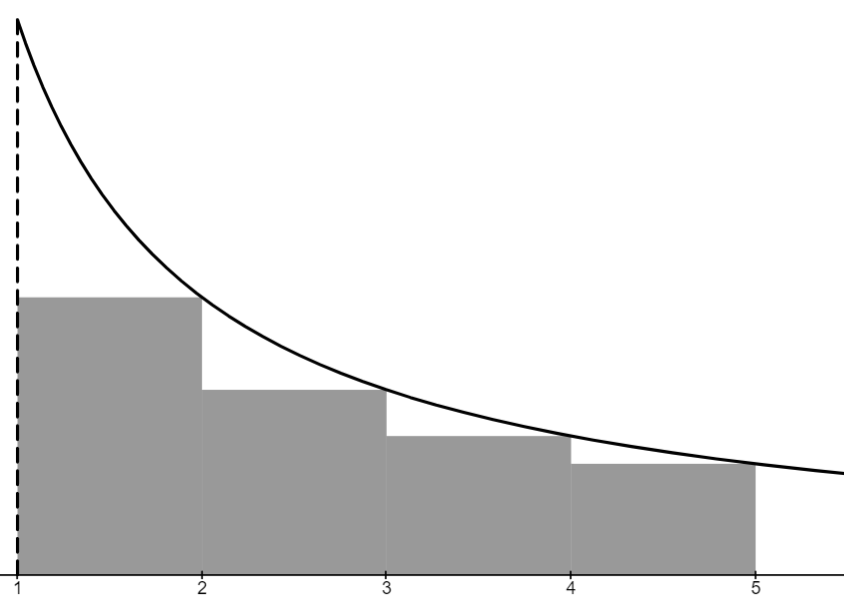
\includegraphics[width = 7 cm]{assets/series-left.png}
        \subcaption[]{Снизу} \label{fig:image1}
    \end{minipage}
    \hfill
    \begin{minipage}{0.45\textwidth}
        \centering
        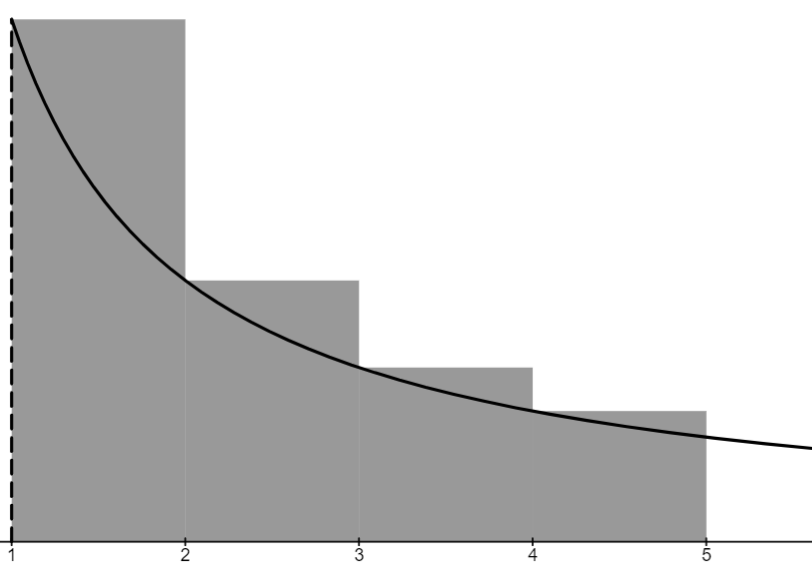
\includegraphics[width = 7 cm]{assets/series-right.png}
        \subcaption[]{Сверху} \label{fig:image2}
    \end{minipage}
\end{figure}
Теперь подробнее, что нам дает такое разбиение: (на примере левой картинки)
$$\integral{1}{+\infty}f(x) = \sum\limits_{k=1}^\infty \integral{k}{k+1}f(x)\geq \sum\limits_{k=1}^\infty \integral{k}{k+1}f(k+1) \geq \sum\limits_{n=2}^{N}f(n) $$
Доказав аналогичное неравенство для левого получим:
$$\sum\limits_{n=1}^{N} f(n)\geq \integral{1}{N} f(x) dx\geq \sum\limits_{n=2}^{N}f(n)$$
А отсюда уже следует равносильность схождения.

\hfill Q.E.D.

\textbf{Замечание:}  ФУНКЦИЯ ДОЛЖНА  БЫТЬ МОНОТОННА.

\textbf{Пример:} 
$$\sum\limits_{n=2}^{+\infty} \cfrac{1}{n^p (\ln n)^q}$$
Как мы показывали ранее мы знаем, когда соотв. интеграл сходится и расходится.


\deff{Абсолютная сходимость.}

$a_n$ - любого знака. $\sum\limits_{n=1}^{+\infty}$ --- абсолютная сходимость если:
\begin{enumerate}
    \item $\sum a_n$ - сходится
    \item $\sum |a_n|$ - сходится
\end{enumerate}

\textbf{Пример:}
$$\cfrac{1}{1+x^2}\leq 1 - x^2  + x^4 - \ldots (-1)^N x^{2N} + \cfrac{(-1)^{N+1}x^{2N+2}}{1+x^2}$$
Проинтегрируем по $[0,1]$, получим:
$$\cfrac{\pi}{4}= 1 -\cfrac{1}{3} + \cfrac{1}{5}+\ldots +\cfrac{(-1)^N}{2N+1}+\integral{0}{1}\cfrac{(-1)^{N+1}x^{2N+2}}{1+x^2}dx$$
Интеграл справа по модулю $\leq$ %todo 28

Ряд $\sum\limits_{n=0}^{+\infty}\cfrac{(-1)^n}{2n+1}$ - не сходим абсолютно

%todo: 30 минута лекции прослушать что тут говорил кохась и выписаьб

Такая формула называется суммой \deff{Грегори-Лейбница}. %todo: мб подумать

\thmm{Теорема.}

$a_n$ --- любого знака. Тогда эквивалентно:
\begin{enumerate}
    \item $\sum\limits_{}a_n$ - абсолютная сходимость.
    \item $\sum\limits_{}|a_n|$ - сходится.
    \item $\sum a_n^+, \sum a_n^-$ - оба сходятся. Где $a_n^+ = \max(a_n,0), a^-_n= \max(-a_n,0)$
\end{enumerate}

\textbf{Доказательство:} смотри теорему в интегралах

\pagebreak
\subsection{Сходимость рядом с произвольными знаками слагаемых}

\thmm{{Теорема (Признак Лейбница)}}

$c_1 \geq c_2 \geq \ldots \geq 0$ (т.е монотонность). Пусть $c_n \rightarrow 0 $. Тогда $\sum\limits_{n=1}^{+\infty} (-1)^{n+1} c_n$ - сходится.

\textbf{Доказательство:}

%37 минут рисунок

И давайте все синие квадратики подвинем налево. Тогда мы получим, что такая сумма будет ограничена. Но мы доказали, что $(c_1-c_2) +(c_3-c_4) + \ldots$  сходится.  Осталось проверить нечетные частичные суммы. $S_{2n+1} =S_{2n}+ c_{2n+1}$ и именно если $c\rightarrow 0 $, то $S_{2n+1}$ стремится к тому же и мы победили.

\textbf{Более формальное доказательство}:

Пусть $S_{2k}  = c_1-c_2 + \ldots +c_{2k-1} - c_{2k}$. Тогда посмотрим на четные суммы:

\begin{enumerate}
    \item $S_{2k}\leq S_{2k+2}$, тк добавили что-то неотрицательное.
    \item $S_{2k}\leq c_1: S_{2k} = c_1-(c_2-c_3)-(c_4-c_5) - (c_{2k-2}-c_{2k-1})-c_{2k}\leq c_1$
\end{enumerate}

Значит существует предел $S_{2k}$. И используйте концовку прошлой.

\hfill Q.E.D.

\thmm{Секретное приложение к признаку Лейбница}

$c_1\geq c_2 \geq \ldots \geq 0  $, $c_n\rightarrow 0 $

$|\sum\limits_{n=N}^{+\infty} (-1)^{n+1}c_n|\leq c_N$

\textbf{Доказательство:} см. теорему выше.

\textbf{Пример:}
\begin{enumerate}
    \item $\sum \cfrac{(-1)^n}{n + \sin n}$ сходится по признаку Лейбница
    \item $\sum\limits_{n=2}^{+\infty}\cfrac{(-1)^n}{n +(-1)^n}$ этот ряд не удовл. признаку Лейбница, тк не монотонна 
\end{enumerate}

\textbf{Очень грустная картинка.}
%todo: вставить грустную картинку   1.04

\deff{Преобразование Абеля (суммирование по частям)}.

$\sum\limits_{n=1}^{N} a_n b_n = A_N b_N + \sum\limits_{n=1}^{N-1}A_n(b_n-b_{n+1})$, где $A_n = a_1 + \ldots + a_n$

\textbf{Доказательство:} Раскройте сумму и получите magic. (не забудьте проверить края)

\thmm{Теорема (признак Абеля и Дирихле)}

\begin{enumerate}
    \item
    \begin{enumerate}
        \item  Пусть частичные суммы последовательности $a_n$ - ограниченны: $\exists C_A: \forall n: a_1 + \ldots + a_n \leq C_A$.
         \item Пусть $b_n$ - монотонна, $b_n\rightarrow 0 $
    
    \end{enumerate}
     Тогда $\sum\limits_{n=1}^{+\infty}a_nb_n$ - сходится
  
   \item
   \begin{enumerate}
       \item Ряд $\sum a_n$ - сходится.
        \item $b_n$ - монотонна и ограничена. $\exists C_B: \forall $
   \end{enumerate}
    Тогда $\sum\limits_{n=1}^{+\infty}a_nb_n$ - сходится.
   
\end{enumerate}

\textbf{Доказательство:}

\begin{enumerate}
    \item $\sum\limits_{n=1}^N a_n b_n =A_n b_n + \sum\limits_{n=1}^{N-1} A(b_n-b_{n+1})$

$A_N$ - ограниченная и $b_N$ - бесконечно малая.

Ряд $\sum\limits_{n=1}^{+\infty} A_n (b_n-b_{n+1})$ - сходится, потому что он сходится абсолютно. А абсолютно он сходится, потому что:
$$\sum\limits_{n=1}^N |A_n||b_n-b_{n+1}|\leq C_A \sum|b_n-b_{n+1}|$$
- разности под модулем одного и того же знака, поэтому 
$$= C_A|b_1-b_{N+1}|\leq C_A \cdot 2 C_B$$
\item
$\exists$ кон. $\lim\limits_{n\rightarrow + \infty} b_n =\beta$. Разложу ряд и получу: $$\sum\limits_{n=1}^{+\infty}a_n b_n = \sum\limits_{n=1}^{+\infty} a_n \beta + \sum\limits_{n=1}^{+\infty}a_n(b_n-\beta)$$
Правильна ли формула? Не всегда, только если пределы есть.

Заметим, что $\sum\limits_{n=1}^{+\infty}a_n \beta$ сходится по усл. $1$. А вторая сумма сходится по признаку Дирихле (первому пункту нашей теоеремы). Откуда имметт предел и мы победили.
\end{enumerate}

\hfill Q.E.D.

\textbf{Пример:}
$$\sum\limits_{n=1}^{+\infty}\cfrac{\sin n}{n^{\alpha}}, \alpha >0$$
$$|\sin 1 + \sin 2+ \ldots + \sin n| = |\Im (e^i + e^{2i} + \ldots + e^{ni})| \leq \Im |e^i\cfrac{e^{ni}-1}{e^i-1}| \leq \cfrac{2}{e^{i}-1} = C_A$$
Откуда ограничены частичные суммы и $b_n = \cfrac{1}{n^{\alpha}}$ монотонна и $b_n\rightarrow 0 $, то выполнен признак Дирихле, откуда победили.

Пример: смерть монстра  %2.10 примерно

\pagebreak
\subsection{Свойства сходящихся рядов.}

Сюжет $I$ --- группировка слагаемых.

\textbf{3 прикола:}
$$1- 1 + 1 -\ldots \rightarrow ???$$
$$(1-1)+(1-1) + \ldots \rightarrow 0$$
$$1 + (-1 + 1) + \ldots \rightarrow 1$$

Так что группировка если работает, то работает очень хитро.

$\sum a_k = (a_1 + \ldots + a_{n_1}) + (a_{n_1+1}+\ldots + a_{n_2})+\ldots$. И теперь я каждую скобоку заменю на $b_i$. 

\thmm{Теорема}

Используя обозначения выше:
\begin{enumerate}
    \item $\sum a_k$ - сходится. Тогда $\sum b_k$ - сходится  и имеет ту же сумму.
    \item $\forall k: a_k\geq 0$, то $\sum a_k, \sum b_k$ имеют одинаковые суммы (или одновременно расходятся)
\end{enumerate}

\textbf{Доказательство:}

$S_k^{(b)} = S^{(a)}_{n_k}$


\hfill Q.E.D.

\deff{def:} $\sum a_k,  \sum b_k$. Ряд $(B)$ - \deff{перестановка} ряда $A$, если $\exists \omega: \N \rightarrow \N$  биекция и $b_k = a_{\omega(k)}$.

\thmm{Теорема:}

Ряд $(A)$ - абс. сходится $\Rightarrow$ Ряд $(B)$ абс. сходится и имеет ту же самую сумму.

\textbf{Доказательство:}

1) Рассмотрим случай $\forall k: a_k \geq 0$.  Посмотрим на какую-то частичную сумму $B$:
$$S_n^{(B)} = b_1 + \ldots + b_n = a_{\omega(1)} + a_{\omega(2)} + \ldots + a_{\omega(n)}$$
Возьмем самую большую омегу $W = \max(w(1),\ldots,w(n))$. 

Заметим, что сумма $a_{\omega(i)}$, будет меньше $S^{(A)}_{W}$, потому что из суммы $S^{(A)}_{W}$ (возможно) выкинули какие-то элементы и получили нашу сумму(а элементы положительные).

$S_n^{(B)}\leq S_W^{(A)}$. Устремим в бесконечность и получим $S^{(B)}\leq S^{(A)}$.

Аналогично для $S^{(A)}\leq S^{(B)}$ (обратная перестановка).

Откуда для неотрицательных рядов при перестановке сумма не меняется.

2) Вернемся к общему случаю, $a_n$ - произвольного знака.

Посмотрим на $a_n^+, a_n^-$, они перестановки $b_n^+, b_n^-$.

По первому пункту $\sum a_n^+ = \sum b_n^+, \sum a_n^- = \sum b_n^-$, ну и понятно что тогда ряд $b$ абсолютно сходится

\hfill Q.E.D

\thmm{Теорема (Риман)}

$\sum a_n$ - сходится, не абсолютно. Тогда:

\begin{enumerate}
    \item $\forall S \in \overline{R}: \exists$ перестановка ряда $a_n: \sum b_n = S$
    \item $\exists$ перестановка: $\not \exists \lim\limits_{n\rightarrow + \infty}S_n^{(b)}$
\end{enumerate}

\textbf{Доказательство:}

Разобьем  наши элементы на две кучки: с положительными и отрицательными элементами ряда. Они обе бесконечные, так как ряд не сходится абсолютно.

Хочу ряд с суммой $2025$

Чтобы набрать сумму конечную сумму $2025$ будем действовать следующим образом:
\begin{enumerate}
    \item берем элементы с наименьшими индексами из положительной кучки, пока сумма впервые не станет больше $2025$.
    \item берем элементы с наименьшими индексами из отрицательной кучки, пока сумма впервые не станет меньше $2025$.
    \item Возвращаемся к пункту 1
\end{enumerate}

Пересекать $2025$ мы будем каждый раз, но при этом ряд сходится, поэтому каждый раз отклонение от $2025$ будет все меньше и меньше, т.е. в пределе ряд будет ровно $2025$.

Чтобы дойти до бесконечности, каждый раз увеличивайте подъем, а чтобы не получить предела поднимайтесь выше $2025$, опускайтесь ниже $2006$.

\hfill Q.E.D.

\textbf{Суммируемое семейство чисел.}

\deff{def:} $\Omega$ - счетное множество $(a_w)_{w\in \Omega}$, $a_\omega \geq 0$ при всех $w$

 $\sum\limits_{w \in \Omega} a_w = \sup\limits_{W\in \Omega}(\sum\limits_{w \in W} a_w) \in \overline{R}$, где $W$ - конечные множества.

Или можно еще вводить по-другому: $\varphi: \N \rightarrow \Omega$ - биекция, то тогда $\sum\limits_{n=1}^{+\infty}a_{\varphi(n)}=S$ 

\deff{def:} $\Omega$ - счетное $(a_w)_{w\in \Omega}$ - \deff{суммируемое семейство}, если $\sum\limits_{w\in \Omega} |a_w| < + \infty$

\thmm{Теорема.}

$(a_w)_{w\in \Omega}$ - сумм. семейство. Тогда:
$$\forall \varphi \N \rightarrow \Omega : \sum\limits_{n=1}^{+\infty} a_{\varphi(n)} = \sum_{w\in \Omega} a_w^+-\sum\limits_{w\in \Omega}a_w^-$$

\textbf{Доказательство:} очевидно из Теоремы о перестановке слагаемых.

\deff{def:} \deff{Произведение рядов} $(\sum a_n) (\sum b_k)$

$\gamma: \N \rightarrow \N \times \N$, $n \rightarrow (\varphi(n), \psi(n))$

Ряд $\sum\limits_{n=1}^\infty a_{\varphi(n)}b_{\psi(n)}$ называется \deff{произведением ($\gamma$ - произведением)}.

\thmm{Теорема (Коши)}

Пусть $\sum a_n = A, \sum b_n = B$, где $A,B \in \R$ и оба ряда сходятся абсолютно.

Тогда $\forall \gamma $ произведение  $\sum\limits_{n=1}^\infty a_{\varphi(n)}b_{\psi(n)}$ сходится абсолютно и к сумме $AB$.

\textbf{Доказательство:}

$\sum |a_n| = A^* \in \R, \sum|b_n|=B^*\in \R$. Проверим: $\sum a_{\varphi(n)}b_{\psi(n)}$ - абсолютно сходится.
$$\sum_{n=1}^N |a_{\psi(n)}b_{\psi(n)}|\leq \left(\sum\limits_{n=1}^K |a_{\varphi(n)}|\right)\left( \sum\limits_{n=1}^L |b_{\varphi(n)}|\right)\leq A^*\cdot B^*$$
Сходимость теперь есть. А теперь благодаря прошлой теореме по суммируемым семействам получаем, что нам не важно как мы умножаем!

Чтобы показать, что сумма ряда сходится, будем смотреть на суммы по \uline{квадратам}: 
$$\sum\limits_{1\leq k\leq n ; 1 \leq l \leq n} S_N^{(a)}S_N^{(b)} \rightarrow AB$$

\hfill Q.E.D.




